\documentclass[a4paper]{article}
\usepackage[margin=19mm]{geometry}
\usepackage[T1]{fontenc}
\usepackage{lmodern,microtype}
\usepackage{amsmath,amssymb,graphicx,booktabs,array,adjustbox,xurl}
\usepackage[hidelinks]{hyperref}
\newcommand{\Fprobe}{\mathcal{F}}
\newcommand{\ind}{\mathbf{1}}
\renewcommand{\thesection}{S\arabic{section}}
\renewcommand{\thetable}{S\arabic{table}}
\renewcommand{\thefigure}{S\arabic{figure}}
\title{Supplementary Materials for: Audit Feedback, Decisions, and Explanations in LLM Trading Agents}
\author{Aldan Jay and Rafael Berlanga}
\renewcommand{\today}{\mbox{}}
\begin{document}
\maketitle
These materials accompany the research Article. Registered and exploratory analyses remain distinct; no new responses were collected. The main paper retains the design and SCI decomposition figures and the primary-model results with a compact replication summary.

\section{Detailed materials and methods}\label{supp:methods}
The confirmatory phase compares five conditions across three models (the main design figure). A seed fixes the random draws used in a run. The primary model is \texttt{deepseek-v4-flash}, with seeds 200--219. The replication models are \path{anthropic/claude-haiku-5.5} and \path{openai/gpt-6-luna}, with seeds 200--209 each. Every seed is crossed with all five conditions. Development uses only seeds 100--101 and is excluded from confirmation. We measure intervention-defined process alignment alongside environmental fidelity. The primary post-switch window is ticks 20--39, the fixed sensitivity window is 10--39, and all-tick summaries cover 0--39. These windows retain regime switches and stale messages. We did not choose a washout period after examining outcomes.


\subsection{Market environment and temporal ordering}
We use a synthetic market with one asset. In plain terms, each return combines the active driver, order imbalance, and noise, and the next price applies that return to the current price. Formally, let $g_t\in\{\mathrm{news},\mathrm{momentum}\}$ denote the active fundamental driver and $x_{g_t,t}$ its observed value. Requested signed sizes determine imbalance. The market updates according to
\begin{equation}
\begin{aligned}
 I_t&=\frac{\sum_{i=1}^{N}s_{it}q_{it}}{5N},\qquad
 r_t=0.02x_{g_t,t}+0.03I_t+\epsilon_t,\\
 \epsilon_t&\sim\mathcal{N}(0,0.005^2),\qquad
 P_{t+1}=\max\{50,P_t(1+r_t)\},\quad P_0=100,
\end{aligned}
 \label{eq:market}
\end{equation}
Here $s_{it}=+1$ for buy and $-1$ for sell, and $N=6$ in the confirmatory phase. The ground-truth driver controls the \emph{fundamental component} of returns. Aggregate orders and residual noise also affect realized returns. Momentum is generated as a signal rather than computed from past prices.

At each tick, an independent latent signal $z_t\sim\mathcal{N}(0,1)$ enters the active feature with independent noise of standard deviation 0.7. The inactive news/momentum feature is independent noise with standard deviation 0.7. Volume is $1+0.3\mathcal{N}(0,1)$; spread is uniform on $[0.004,0.03]$; orderflow is $0.3\,\mathrm{momentum}+\mathcal{N}(0,0.6^2)$; sentiment is $0.3\,\mathrm{news}+\mathcal{N}(0,0.6^2)$. Distractors are features outside the fundamental term, although they can correlate with its driver. Features are stored at three decimals, except spread at four. Even seeds start in news and odd seeds in momentum. Regimes switch at ticks 10, 20, and 30.

Agents observe the current features and completed history before submitting orders. The market then computes the return and new price. After an audited failure in the confirmatory phase, a fine reduces cash and position alike before the selected trade settles. Both are multiplied by 0.90 at the post-step price. In intuitive terms, the fine applies to everything the agent owns, not only its cash. Formally, it equals 10\% of total marked wealth, $W=\mathrm{cash}+\mathrm{position}\times P_{t+1}$, even when cash alone is insufficient. Purchases require cash and sales require inventory; borrowing and short sales are not allowed. Requested sizes still enter imbalance. Re-asks never submit orders, change feedback, or advance history.

Paired seeds give every condition the same exogenous feature draws, residual shocks, and regime schedules for a given seed. Endogenous returns, price paths, portfolio states, and later observed return histories can still differ because agents act differently. Treatment effects include these feedback paths. Pairing does not make the complete market states identical.

\subsection{Agents, portfolios, and prompts}
The confirmatory phase crosses three fixed mandates (cautious, balanced, and growth) with two starting portfolios: cash USD 4000 and position 20, or cash USD 1000 and position 50. We use nominal USD to present the synthetic account units. Each agent begins at wealth USD 6000 at an initial asset price of USD 100. These simulated balances are separate from provider expenditures. Assignments remain identical across seeds, conditions, and models. Mandates change risk and sizing instructions. They do not create independent statistical replications or human-like personalities.

Each response must use strict JSON, a structured text format, with action buy/sell, integer size 1--10, and an ordered unique list of zero to two reasons drawn from momentum, spread, volume, news, orderflow, and sentiment. Extra keys, fabricated actions, coercion, and invalid-response retries are disallowed. There is no hold action. Reasoning/thinking output is disabled, and the maximum output length is 512 tokens. These rules constrain the response format but do not eliminate unobserved computation.

The system message contains the common instruction, institutional rules, and response schema. The user message contains the persona mandate, latest audit feedback if present, portfolio state, four completed feature--return pairs, and finally the current features. Current features use a fixed order and four-decimal formatting. The static prefix precedes dynamic material to facilitate prompt caching. We do not hypothesize a behavioral benefit from this ordering. All five rule paragraphs share the same true-driver framing and differ only in the final feedback-description sentence. Label and placebo have identical rule descriptions and disclosed-label wording. Supplementary Section~\ref{app:reproducibility} gives the complete verbatim prompts, feedback templates, rendered examples, response schema, and persona mandates.

\subsection{Feedback conditions}
An environmental audit checks whether the base reasons include the current fundamental driver. In all audited conditions, each decision has audit probability 0.30, and a failed audit incurs the total-wealth fine. The audit evaluates environmental fidelity rather than process precision. Both passing and failing audits supply feedback after the action. That feedback first appears in the next prompt and persists unchanged until the next audit, including across switches.
\begin{table}[tbp]
\caption{Confirmatory phase conditions. All conditions require explanations and use identical shared institutional text. A placebo message is deliberate false information, not an inert control.}
\label{tab:design}
\centering\footnotesize
\begin{tabular}{llp{.62\linewidth}}
\toprule
Condition & Audit rate & Feedback content \\
\midrule
naive & 0 & No verdict, fine, or additional information \\
punitive & 0.30 & Environmental verdict and actual fine; no label or statistics \\
label & 0.30 & Verdict/fine and the true driver at the audited tick \\
evidence & 0.30 & Verdict/fine and recent correlations for every feature; no named driver \\
placebo & 0.30 & Truth-based verdict/fine and the opposite driver label \\
\bottomrule
\end{tabular}
\end{table}

The placebo verdict remains truth-based, but its disclosed label is false at audit time. This intentionally conflicting message tests false authority. A persisted true label can become stale, and a persisted placebo label can become correct after a switch. We determine prompt exposure from logs rather than responses.

Evidence reports Pearson correlations, which summarize linear association, between each of all six features and realized returns over the last eight completed ticks. The window includes the audited tick, and features appear in fixed order. Feedback reports sample sizes and four-decimal coefficients. Fewer than two observations or zero variance yields ``unavailable''. The builder has no regime input, ranking, threshold, or preferred feature. Its associations include endogenous price impact and noise and can mix regimes. Evidence also summarizes a longer history than the four completed rows given to every agent. This longer history is part of the intervention, so evidence-versus-label is not a pure wording comparison.

\subsection{Preregistration, calibration, and amendments}\label{sec:amendments}
The original plan replaced features with adversarial extremes directed against the base action. Its pilot failed the ceiling gate: DeepSeek naive true-driver flips were 109/114 (0.956), above the 0.95 ceiling. The PI stopped that pilot. Amendment 1 prospectively replaced the instrument with sign reversal after calibration on dev seeds 100--101. Calibration compared zeroing, sign reversal, adverse shifts of one/two feature standard deviations, and the original extremes. The fixed rule required every model's pooled naive true-driver rate to lie in $[0.10,0.90]$. It maximized the minimum true-minus-non-driver discrimination across models, where discrimination is the difference between those flip rates. Differences within 0.02 were ties in a fixed perturbation order, and the best minimum had to be at least 0.15. Sign reversal was selected with minimum discrimination 0.184. This procedure calibrates a measurement instrument; it is not a confirmatory hypothesis test.

Independent dev null re-asks yielded naive flip rates of 0.043, 0.041, and 0.053 for DeepSeek, Haiku, and Luna. Net true-driver rates remained eligible, with minimum discrimination 0.197 in those separate noise runs. A common null rate cancels when subtracted from both true and non-driver rates before taking their difference. This subtraction does not remove all measurement error. Label outcomes did not enter the selection rule, but the PI and coordinator had seen descriptive dev label dependence exceeding naive. That exposure and the reuse of dev seeds for calibration and noise assessment limit the independence of development evidence. None of these observations is pooled with confirmation. The development reports retain and disclose extra dev null calls and quarantined overlapping-run artifacts.

Amendment 1 also added one null re-ask on a random 20\% of counterfactual-selected decisions, condition-specific noise monitoring, provider pins, and the temperature exceptions below. It removed the optional Qwen allocation on cost grounds. The four primary contrasts, H1--H5, directions, windows, aggregation, and inferential thresholds remained unchanged. The PI answered yes to all eight amended questions before confirmation.

Amendment 2 changed only budget operations after collection began. Higher Haiku costs prompted an account top-up and moved the OpenRouter procedural stop from USD 7.400 to USD 7.950, with the review reserve funded separately. The hard USD 8 provider cap remained in force, as did the DeepSeek USD 7.000 pause. No confirmatory outcome was inspected for that decision. The plan was refrozen with both amendments. Models, seeds, conditions, measurement, hypotheses, and analysis were unchanged. The renewed frozen plan has SHA-256 \path{dd8eaf872b37593433b3168725962937}\allowbreak\path{394d1b5d1c4ef005fe415534c37235a1}, recorded in \path{preregistration/FROZEN.json} of the public repository.

\subsection{Counterfactual sign-flip instrument and noise monitoring}\label{sec:noise}
An independent Bernoulli(0.50) measurement mask randomly selects decisions before responses and is paired across conditions. For each valid selected base response, two re-asks retain its exact prompt state and settings. They replace only the current news or momentum value $v$ by $-v$. The intervention direction is independent of the base action, and zero remains zero without resampling. Portfolio, feedback, history, and other feature values remain fixed. We ignore counterfactual reasons. The probe measures whether this input intervention changes the action, including through a nonlinear response. It does not test trade-size explanations, necessary causation, or the other four features.

The amended design uses one byte-identical null re-ask on 20\% of sampled decisions to estimate response variability. Byte-identical means that every character and setting remains unchanged. Primary dependence and gap tests use raw flips. A secondary sensitivity subtracts the pooled model-by-condition null action-flip rate from pooled feature/driver rates, without clipping adjusted values to a fixed range. Pooling combines responses rather than averaging seed-level estimates. This adjustment does not redefine decision-level precision, recall, or SCI. The registered noise adjustment subtracts pooled all-tick model-by-condition null rates from pooled feature/driver rates. It is not a paired-seed adjustment of the primary contrasts or SCI. Raw flips therefore combine intervention sensitivity with re-ask variability. Null-rate intervals are descriptive Wilson intervals over responses and do not account for seed clustering. Section~\ref{sec:protocol} reports deviations in realization of the null mask.

\subsection{Metrics and estimands}\label{sec:metrics}
In intuitive terms, we compare what the agent cites with what changes its action under the probe. Indicator notation records whether a condition holds. For decision $j$, let $a_j$ be the base action, $a_j^{(f)}$ its action after feature $f$ is sign-reversed, $R_j$ the base reasons, and $g_j$ the current true fundamental driver. With $\Fprobe=\{\mathrm{news},\mathrm{momentum}\}$, define
\begin{equation}
 E_j=\ind[g_j\in R_j],\qquad d_{jf}=\ind[a_j^{(f)}\ne a_j],\qquad
 C_j=R_j\cap\Fprobe,\qquad D_j=\{f\in\Fprobe:d_{jf}=1\}.
\end{equation}
Environmental fidelity $E_j$ uses valid base responses. True-driver dependence is $d_{j,g_j}$ and non-driver dependence is $d_{j,\bar g_j}$, where $\bar g_j$ denotes the other feature. Process precision asks how many cited probe features also change the action when reversed. Process recall asks how many action-changing probe features were cited. The unconditional alignment score compares the complete citation and dependence sets. For complete valid measurements,
\begin{equation}
 P_j=\frac{|C_j\cap D_j|}{|C_j|}\ (|C_j|>0),\qquad
 Q_j=\frac{|C_j\cap D_j|}{|D_j|}\ (|D_j|>0),\qquad
 U_j=1-\frac{|C_j\triangle D_j|}{2}.
 \label{eq:process}
\end{equation}
Precision $P_j$ and recall $Q_j$ measure citation agreement with this particular sign-flip probe, not ground-truth process accuracy. They remain undefined at zero denominators and apply only within $\Fprobe$. An unprobed distractor citation is not declared a false positive. The released analysis reports structural undefined scores separately from parse/transport failures, together with citation coverage and dependence-set sizes. The secondary unconditional alignment score $U_j$ counts two empty sets as agreement and therefore answers a different question.

If the actual prompt contains label $L_j$, adoption is $A_j=\ind[L_j\in R_j]$, conditional on exposure. We report cited/exposed counts and proportions separately for currently correct and stale labels. Intuitively, SCI asks whether a citation changes more or less than the corresponding sign-flip dependence. For matched eligible measured coordinates $J_{sc}$ in seed $s$, condition $c$, and naive reference $n$, define the strategic-compliance index (SCI), or explanation--behavior gap, by
\begin{align}
 \mathrm{SCI}_s(c;X)
 &=\frac{1}{|J_{sc}|}\sum_{j\in J_{sc}}
 \left(\ind[X_j\in R_{cj}]-\ind[X_j\in R_{nj}]\right)\nonumber\\
 &\quad-\frac{1}{|J_{sc}|}\sum_{j\in J_{sc}}
 \left(d_{cj,X_j}-d_{nj,X_j}\right).
 \label{eq:sci}
\end{align}
SCI is an operational difference between citation change and sign-flip-dependence change. Its scale and zero point are not externally validated measures of explanation completeness, concealment, or intent.

Primary label SCI selects $X_j=g_j$ and primary placebo SCI selects $X_j=\bar g_j$ at every primary-window coordinate, including before exposure. These intention-to-treat (ITT) selectors include coordinates regardless of whether an audit occurred, avoiding selection on treatment-dependent audits. A positive SCI means citation increased more than measured dependence. A negative SCI means dependence increased more. Neither sign establishes a motive, deliberate strategy, or deception. Secondary exposure SCI instead applies the actual possibly stale $L_{cj}$ to both paired prompts.

Within each seed, process scores average defined decision-level values rather than pooled numerator/denominator ratios. Contrasts use common tick/agent coordinates with valid base responses and both counterfactuals in both conditions. Precision contrasts also require a defined score in both conditions. This restriction means precision's estimand can depend on treatment. Each eligible seed receives equal weight. We report all-available condition means separately; they need not equal the means underlying a contrast or SCI component.

\subsection{Hypotheses and statistical plan}\label{sec:statistics}
The confirmatory-phase hypotheses remain as registered. H1 predicts positive evidence-minus-naive gains in both precision and true-driver dependence. Evidence's dependence advantage over punitive is secondary. H2 predicts greater environmental fidelity/true-driver citation under label, a positive label precision contrast, and a larger precision gain under evidence than label. The precision comparisons are secondary. H3 predicts a positive label SCI. H4 predicts a positive placebo SCI, increased false citation, and lower environmental fidelity than label. H5 predicts a smaller precision gain under punitive than evidence. A nonsignificant punitive comparison cannot establish equivalence. P2 compares the complete evidence audit package with naive, and P4 compares the placebo audit package with naive. Neither isolates numerical content or label falsity.

The sole DeepSeek primary family contains four two-sided paired $t$ tests of equal-seed differences: P1 evidence-minus-naive precision, P2 evidence-minus-naive true-driver dependence, P3 label SCI, and P4 placebo SCI. A paired test compares conditions within the same seed. The family uses $\alpha=0.05$ with four-slot Holm step-down correction regardless of effect sign. Holm correction adjusts $p$ values sequentially to account for multiple comparisons. Missing/untestable contrasts retain $p=1$. A two-sided rejection opposite to prediction does not support a positive hypothesis. Each replication uses its own four-slot correction, without pooling models or correcting across models. Replications cannot rescue a failed primary prediction. H2/H5 and the secondary components of H4 have no additional confirmatory rejection rule.

The released analysis reports paired differences, paired SD and $d_z=\bar\Delta/\mathrm{SD}(\Delta_s)$, sample sizes, and raw/adjusted $p$ values. Paired SD is the standard deviation of seed-level differences. Descriptive 95\% intervals come from 10,000 paired-seed percentile bootstrap resamples with RNG seed 20261026. Bootstrapping repeatedly resamples seeds to describe uncertainty. These intervals are not simultaneous confidence intervals and do not override the registered $t$ test. The prospective standardized minimum detectable effects at 80\% power and the conservative first Holm threshold 0.0125 were $d_z=0.8146$ for 20 seeds and 1.2843 for 10. Small effects can be missed. More agents or re-asks do not increase the replication count.

Registered sensitivities include all paired-seed sign permutations and decision-level regressions with condition, tick, regime, persona, initial inventory, and seed fixed effects. Fixed effects allow separate intercepts for each category. Standard errors cluster by market seed across all conditions, using CR1 finite-cluster correction and $G-1$ reference degrees of freedom. A null-imposed Rademacher wild bootstrap uses 9,999 draws. These diagnostic tests do not create a replacement primary family. Pooled Gaussian run-mean mixed models include condition, model, and their interaction, with seed and model-by-seed random intercepts, as secondary descriptions. Wilcoxon tests and Cohen's $h$ in the released analysis are exploratory supplements absent from the frozen plan and do not determine verdicts.

All assigned runs remain in the manifest. Primary pairs require complete 40-tick runs and at least one eligible common coordinate. Invalid JSON and exhausted transport retries count as missing; we never fabricate actions. A failed base yields no order. The market advances with available orders and the fixed six-agent denominator. Valid bases with incomplete counterfactuals retain environmental/citation scores but are excluded from complete-case process scores. Missing nulls do not invalidate otherwise valid process measurements. Structural undefined scores remain distinct. The analysis reports worst/best missing-score bounds for unconditional alignment and feature dependence. It also reports denominators and missingness by run, feature, and exposure.

\subsection{Models, transport, and execution safeguards}\label{sec:transport}
DeepSeek used the direct DeepSeek chat-completions transport at temperature zero. Haiku and Luna used OpenRouter pinned respectively to \texttt{anthropic} and \texttt{openai}, with \texttt{allow\_fallbacks:false} and \texttt{data\_collection:deny}. We omitted temperature for both replications because the endpoint listings checked on 27 October 2026 did not advertise support. They therefore used provider-default sampling. The original universal temperature-zero plan does not describe these routes. We logged the returned serving-provider identity. A missing/mismatched provider would be a charged failed call, but no provider mismatch was observed. Model IDs and access dates identify the deployed services, not immutable model weights.

The transport enforced JSON, disabled reasoning/thinking, and logged usage and retries. It allowed at most three identical-payload attempts for transient failures, with delays of one then two seconds. We did not resample valid responses for a preferred action. During development, we evaluated and rejected a free OpenCode CLI route because it added runtime system text, quoted the user payload, and generated title requests. It could not preserve the experimental messages. No OpenCode output enters either confirmatory model cohort.

Independent audit and counterfactual RNG streams use seeds $1000s+7$ and $1000s+17$. RNG means random number generator. The amended null recipe specified a full independent mask from $1000s+29$. Audit masks are paired across audited conditions and counterfactual masks across all conditions. Conditions rotate in order by seed, and all conditions of a seed precede the next seed. Exclusive block locks, bounded concurrency, and a guard validating the freeze commit/hash protect collection. Only the coordinator resumes interrupted blocks. There was no outcome-based stopping or replacement-seed rule. The repository retains code, raw prompts, model/provider metadata, masks, and per-call accounting.

\section{Detailed results and protocol record}\label{supp:results}
\begin{table}[tbp]
\caption{Detailed replication contrasts. Definitions and correction follow the main primary-results table; intervals are descriptive and non-simultaneous.}
\label{tab:replications}
\centering\small
\begin{adjustbox}{max width=\linewidth}
\begin{tabular}{llrrlrrr}
\toprule
Model & Test & $n$ & $\Delta$ & Interval & Raw $p$ & Holm $p$ & $d_z$ \\
\midrule
Haiku & P1 & 10 & 0.0163 & [-0.0362, 0.0642] & 0.5613 & 1.0000 & 0.1907 \\
Haiku & P2 & 10 & -0.0059 & [-0.0609, 0.0531] & 0.8499 & 1.0000 & -0.0616 \\
Haiku & P3 & 10 & -0.0354 & [-0.0892, 0.0210] & 0.2542 & 0.7625 & -0.3852 \\
Haiku & P4 & 10 & -0.0572 & [-0.1045, -0.0039] & 0.0666 & 0.2666 & -0.6596 \\
Luna & P1 & 10 & -0.1198 & [-0.1562, -0.0838] & 0.0002 & 0.0007 & -1.9472 \\
Luna & P2 & 10 & -0.0909 & [-0.1396, -0.0312] & 0.0125 & 0.0376 & -0.9832 \\
Luna & P3 & 10 & -0.0333 & [-0.0845, 0.0252] & 0.2883 & 0.2883 & -0.3568 \\
Luna & P4 & 10 & 0.0404 & [-0.0069, 0.0821] & 0.1272 & 0.2544 & 0.5314 \\
\bottomrule
\end{tabular}
\end{adjustbox}
\end{table}

\subsection{Confirmatory phase (preregistered): completion and primary results}\label{sec:primary}
The confirmatory runs were complete, and every DeepSeek primary estimate opposed its predicted positive direction. All 200 assigned runs were included: 100 DeepSeek runs and 50 each for Haiku and Luna. Every primary contrast retained all 20 or 10 seed pairs. Invalid base decisions across all conditions/ticks numbered 0 for DeepSeek, 6 for Haiku, and 3 for Luna. Missingness does not conceal an incomplete condition or replaced seed (Supplementary Section~\ref{app:coverage}).

The main primary-results table and Supplementary Table~\ref{tab:replications} report all four primary contrasts for all models, and Figure~\ref{fig:forest} displays their intervals. In DeepSeek, P1 evidence-minus-naive precision was $-0.0137$ with an interval spanning zero. P3 label SCI was $-0.0389$ and also inconclusive. Neither result establishes a zero effect. P2 evidence-minus-naive true-driver dependence was $-0.0624$ (Holm $p=0.0140$), and P4 placebo SCI was $-0.1341$ (Holm $p=4.18\times10^{-5}$). Both corrected rejections are opposite to their registered positive predictions.

\begin{figure}[tbp]
\centering
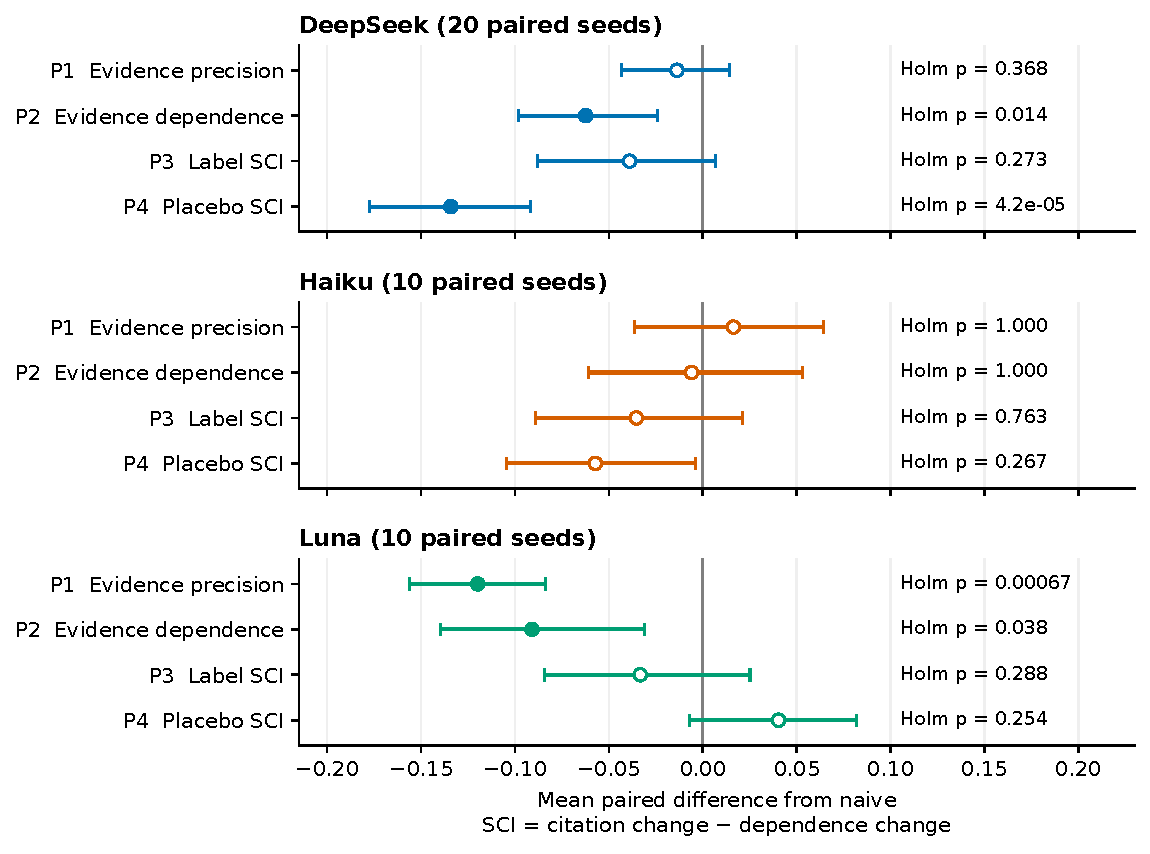
\includegraphics[width=.98\linewidth]{figures/v9/fig2_primary_forest.pdf}
\caption{Four registered contrasts in each model. Points show equal-seed paired differences on common eligible coordinates; bars are descriptive 95\% seed-bootstrap intervals. Filled points mark Holm $p<0.05$ within that model, not interval exclusion alone. Every registered predicted direction was positive. P3 and P4 are differences in citation change minus dependence change.}
\label{fig:forest}
\end{figure}

The SCI decomposition separates citation changes from dependence changes on matched coordinates (the main SCI decomposition figure). For DeepSeek correct labels, true-driver citation increased by 0.0655 and true-driver dependence increased by 0.1044, yielding SCI $-0.0389$. For placebo, opposite-current-driver citation increased by 0.1192 and dependence by 0.2533, yielding SCI $-0.1341$. These paired components use the same coordinates and seed weights as each SCI. Under the registered SCI, placebo increased opposite-driver sign-flip dependence 0.1341 more than opposite-driver citation. This result does not claim deliberate concealment. Correct labels supplied no evidence for the predicted positive gap. The negative, inconclusive SCI cannot rule out all forms of strategic compliance.


\begin{table}[tbp]
\caption{Registered H1--H5 verdicts for the primary DeepSeek model, retained from the confirmatory report. Secondary evidence uses estimates and descriptive, non-simultaneous intervals, without an additional confirmatory rejection rule.}
\label{tab:verdicts}
\centering\footnotesize
\setlength{\tabcolsep}{4pt}
\begin{tabular}{>{\raggedright\arraybackslash}p{.17\linewidth}>{\raggedright\arraybackslash}p{.21\linewidth}>{\raggedright\arraybackslash}p{.55\linewidth}}
\toprule
Hypothesis & Verdict & Evidence \\
\midrule
H1 evidence & not supported & P1 is negative and inconclusive; P2 is negative with Holm rejection, contrary to both predicted positive gains. \\
H2 label & mixed & Environmental fidelity/true citation rises; label precision is negative and inconclusive, and evidence does not outperform label in precision. \\
H3 strategic compliance & not supported & Label SCI is negative and inconclusive; the predicted positive disproportionate citation change is absent. \\
H4 false authority & mixed & Placebo SCI is significantly negative, contrary to the gap prediction; false citation rises and fidelity is below label, as predicted secondarily. \\
H5 punishment & registered secondary direction observed; not confirmatory & Evidence exceeds punitive in precision with a positive descriptive, non-simultaneous interval; punitive is below naive. This is relative advantage, not improvement over naive or punishment equivalence. \\
\bottomrule
\end{tabular}
\end{table}

\subsection{Independent model replications}
The replication models provide no corrected support for a predicted positive primary effect. Haiku had no Holm-significant primary contrast. Its evidence precision estimate was positive ($+0.0163$). Evidence dependence ($-0.0059$), label SCI ($-0.0354$), and placebo SCI ($-0.0572$) were negative and inconclusive under the registered tests. Haiku's placebo bootstrap interval excludes zero, but its paired $t$ test does not reject. The descriptive interval does not override that test.

Luna replicated the negative evidence-dependence effect ($\Delta=-0.0909$, Holm $p=0.0376$) and also showed reduced precision ($\Delta=-0.1198$, Holm $p=0.0007$). Its label SCI was negative and inconclusive ($-0.0333$), while placebo SCI was positive and inconclusive ($+0.0404$). The DeepSeek negative placebo gap therefore does not replicate as a corrected effect across both models. The common negative label estimates show descriptive consistency. They are not evidence of equivalence or a pooled discovery.

\subsection{Instrument validity, noise, and coverage}\label{sec:validity}
The probe passed the pooled flip-rate gate in every model, but regime checks limit its interpretation. All models passed the amended pooled naive true-driver interval $[0.10,0.90]$ (Table~\ref{tab:validity}, Figure~\ref{fig:validity}). True-driver flips were 1363/2421 (0.5630) for DeepSeek, 595/1198 (0.4967) for Haiku, and 660/1196 (0.5518) for Luna. Corresponding true-minus-non-driver discrimination was 0.2012, 0.1845, and 0.1982. These diagnostic response counts are not independent replication counts. Discrimination has no new confirmatory threshold.

The prespecified pooled flip-rate gate shows that the probe is neither near-universally positive nor near-universally negative. It does not establish true-driver discrimination in each regime. In the news regime, discrimination was reversed for DeepSeek ($-0.1157$) and near zero for Haiku ($0.0033$). We therefore interpret outcomes in these strata as sign-flip sensitivity rather than correct or incorrect driver use. Momentum-regime discrimination was positive for both models, and Luna remained positive in both regimes. All strata remain in the preregistered tests without outcome-driven exclusions.

\begin{table}[tbp]
\caption{Naive instrument validity at ticks 0--39. All pooled true-driver rates pass the inclusive [0.10, 0.90] diagnostic. Regime discrimination is descriptive and does not define an exclusion or a further confirmatory gate.}
\label{tab:validity}
\centering\footnotesize
\setlength{\tabcolsep}{4pt}
\begin{adjustbox}{max width=\linewidth}
\begin{tabular}{lllrlrr}
\toprule
Model & Regime & True flips/$n$ & True rate & Non-driver flips/$n$ & Non-driver rate & Difference \\
\midrule
DeepSeek & pooled & 1363/2421 & 0.5630 & 876/2421 & 0.3618 & 0.2012 \\
DeepSeek & news & 491/1219 & 0.4028 & 632/1219 & 0.5185 & -0.1157 \\
DeepSeek & momentum & 872/1202 & 0.7255 & 244/1202 & 0.2030 & 0.5225 \\
Haiku & pooled & 595/1198 & 0.4967 & 374/1198 & 0.3122 & 0.1845 \\
Haiku & news & 243/607 & 0.4003 & 241/607 & 0.3970 & 0.0033 \\
Haiku & momentum & 352/591 & 0.5956 & 133/591 & 0.2250 & 0.3706 \\
Luna & pooled & 660/1196 & 0.5518 & 423/1196 & 0.3537 & 0.1982 \\
Luna & news & 334/606 & 0.5512 & 221/606 & 0.3647 & 0.1865 \\
Luna & momentum & 326/590 & 0.5525 & 202/590 & 0.3424 & 0.2102 \\
\bottomrule
\end{tabular}
\end{adjustbox}
\end{table}

\begin{figure}[tbp]
\centering
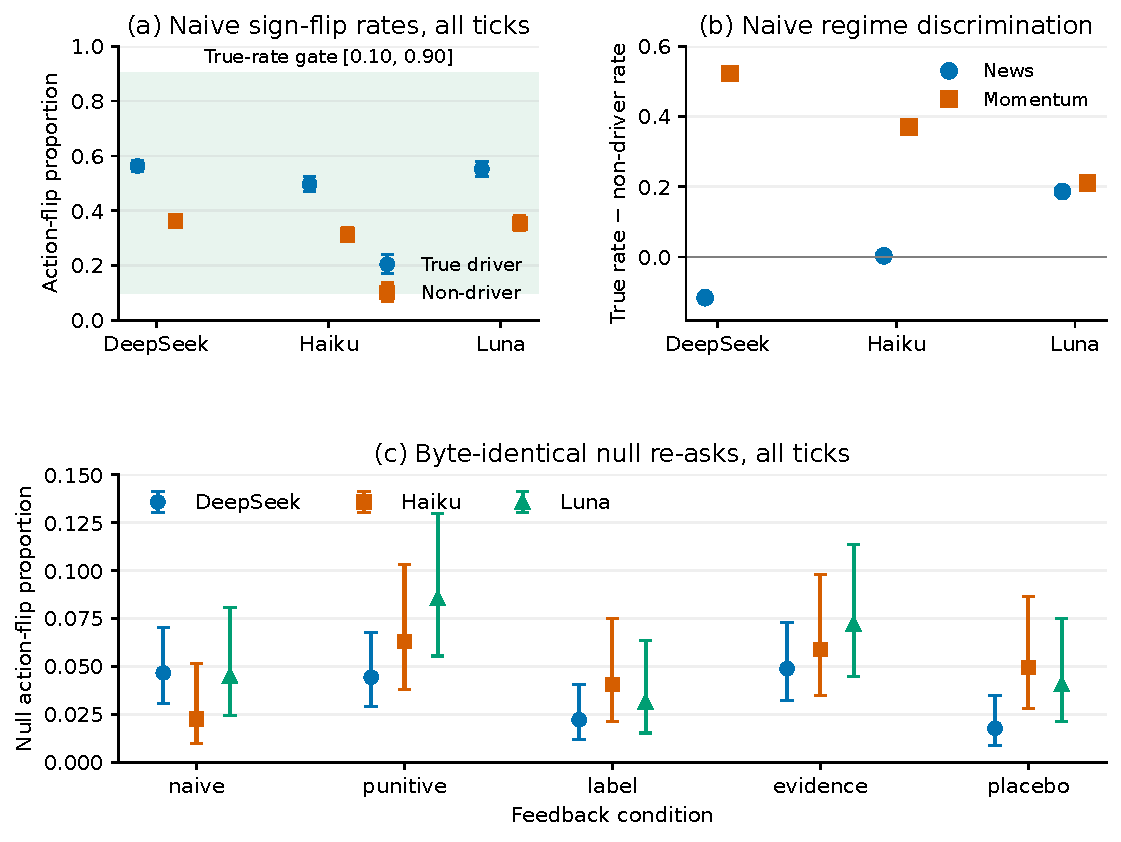
\includegraphics[width=.98\linewidth]{figures/v9/fig4_validity_noise.pdf}
\caption{Instrument and noise diagnostics at ticks 0--39. (a) Pooled naive true/non-driver sign-flip rates, with the amended true-rate gate shaded. (b) Naive discrimination by regime, including DeepSeek's news-regime reversal and Haiku's near-zero news result. (c) Identical-prompt null action-flip rates by model and condition. Wilson intervals in (a,c) are descriptive response-level intervals, not seed-cluster intervals or additional hypothesis tests.}
\label{fig:validity}
\end{figure}

Null flip rates varied by model and condition (Supplementary Table~\ref{tab:noise}). Naive rates were 21/450 (0.0467), 5/222 (0.0225), and 10/222 (0.0450) for DeepSeek, Haiku, and Luna. DeepSeek label/placebo rates were lower, at 10/450 (0.0222) and 8/450 (0.0178). All valid selected nulls were observed. One selected invalid Haiku evidence base was excluded from its null denominator. Primary outcomes remain raw. For illustration, pooled primary-window DeepSeek true-driver rates change from 0.5957 to 0.5490 in naive and from 0.5319 to 0.4830 in evidence after their respective null-rate subtractions. These adjusted pooled rates are not paired equal-seed contrasts and do not redefine SCI, precision, or recall.

Coverage differed across contrasts because some coordinates lacked common support or defined denominators. DeepSeek P1 used 1203 matched coordinates; its other primary tests used 1207. Haiku P1 used 555 and Luna P1 used 582. Every seed pair remained eligible. Supplementary Table~\ref{tab:coverage} reports complete primary-window measurements and undefined precision/recall counts per condition. High conditional recall does not imply comprehensive fidelity. Recall omits empty dependence sets, and precision does not cover unprobed features.

\subsection{Registered sensitivities}\label{sec:sensitivities}
The sensitivity analyses preserve every primary estimate sign, although two raw significance decisions change in the wider window. Paired-seed permutations, covariate-adjusted seed-cluster regressions, and wild-bootstrap sensitivities preserve all primary estimate signs. At the raw 0.05 threshold, they give no significance disagreement with the raw primary-window paired tests (Supplementary Table~\ref{tab:sensitivity}). This is not a second multiplicity-adjusted confirmation. For DeepSeek dependence, permutation $p=0.0060$ and wild $p=0.0051$ support the negative direction descriptively. For DeepSeek placebo SCI, corresponding values are approximately $9.54\times10^{-6}$ and 0.0001. Small cluster counts still limit these diagnostics.

Two raw significance decisions change in the fixed wider window, ticks 10--39. DeepSeek evidence precision becomes $-0.0220$ (raw $p=0.0237$), and Haiku placebo SCI becomes $-0.0613$ (raw $p=0.0021$). Both retain the negative sign, contrary to prediction. The primary family and verdicts remain based on ticks 20--39. The full analysis releases missing-score lower/upper bounds, featurewise missingness, and the other fixed-window sensitivities. We did not select an alternative window or correction for a favorable result.

\subsection{Registered secondary outcomes}\label{sec:secondary}
The secondary outcomes show strong label adoption but no consistent precision benefit from evidence. Table~\ref{tab:secondary} separates secondary estimates from the primary family. All confidence intervals (CI) used in this subsection are descriptive and non-simultaneous. They do not yield confirmatory verdicts. In DeepSeek, label increases environmental fidelity/true-driver citation by 0.0638 (CI [0.0429, 0.0858]) relative to naive. Placebo increases false citation by 0.1058 (CI [0.0792, 0.1337]) and lowers fidelity relative to label by 0.0496 (CI [$-0.0704$, $-0.0283$] for placebo minus label). These components explain the mixed H2/H4 verdicts. Their eligibility sets differ, so they are not the matched SCI citation components.

Evidence exceeds punitive in DeepSeek precision by 0.0328 (CI [0.0023, 0.0654]). This observes H5's registered secondary direction without confirmatory status. Punitive itself is below naive by 0.0468 (CI [$-0.0621$, $-0.0326$]). H5 therefore does not show that numerical feedback helps relative to naive. Its evidence-minus-punitive precision direction is negative and inconclusive in Haiku and negative in Luna. Secondary H5 does not generalize consistently.

\begin{table}[tbp]
\caption{Registered primary-window secondary estimates and descriptive 95\% seed-bootstrap intervals. These are not additional confirmatory discoveries. Exposed analyses select on treatment-dependent feedback and use the actual possibly stale label.}
\label{tab:secondary}
\centering\footnotesize
\setlength{\tabcolsep}{4pt}
\begin{adjustbox}{max width=\linewidth}
\begin{tabular}{p{.34\linewidth}lll}
\toprule
Contrast & DeepSeek & Haiku & Luna \\
\midrule
H2: label $-$ naive, fidelity & 0.0638 [0.0429, 0.0858] & 0.0776 [0.0418, 0.1151] & 0.0726 [0.0492, 0.1009] \\
H2: label $-$ naive, precision & -0.0102 [-0.0416, 0.0212] & 0.0834 [0.0237, 0.1337] & 0.0041 [-0.0457, 0.0579] \\
H2: evidence $-$ label, precision & -0.0038 [-0.0364, 0.0287] & -0.0581 [-0.1132, -0.0002] & -0.1225 [-0.1634, -0.0772] \\
H4: placebo $-$ label, fidelity & -0.0496 [-0.0704, -0.0283] & -0.1802 [-0.2221, -0.1367] & -0.1285 [-0.1733, -0.0808] \\
H4: placebo $-$ naive, false citation & 0.1058 [0.0792, 0.1337] & 0.1208 [0.0567, 0.1808] & 0.1717 [0.1225, 0.2208] \\
H5: evidence $-$ punitive, precision & 0.0328 [0.0023, 0.0654] & -0.0121 [-0.0583, 0.0357] & -0.1027 [-0.1484, -0.0585] \\
H5: punitive $-$ naive, precision & -0.0468 [-0.0621, -0.0326] & 0.0338 [0.0046, 0.0602] & -0.0176 [-0.0508, 0.0144] \\
H1: evidence $-$ punitive, dependence & -0.0805 [-0.1214, -0.0359] & -0.0454 [-0.0851, 0.0020] & -0.0770 [-0.1488, -0.0030] \\
H3: actual-label exposed SCI & -0.2435 [-0.2941, -0.1900] & -0.0655 [-0.1206, -0.0011] & -0.0482 [-0.1329, 0.0337] \\
H4: actual-placebo-label exposed SCI & -0.3169 [-0.3674, -0.2645] & -0.1140 [-0.1632, -0.0650] & -0.0041 [-0.0639, 0.0531] \\
\bottomrule
\end{tabular}
\end{adjustbox}
\end{table}

\begin{table}[tbp]
\caption{All-available primary-window condition means, with equal weight per defined seed. These differ from pair-specific common-support contrasts. $P$: process precision; $Q$: process recall; $U$: unconditional alignment; $d_g$: true-driver dependence; $d_{\bar g}$: non-driver dependence; $E$: environmental fidelity.}
\label{tab:conditions}
\centering\footnotesize
\setlength{\tabcolsep}{4pt}
\begin{adjustbox}{max width=\linewidth}
\begin{tabular}{llrrrrrr}
\toprule
Model & Condition & $P$ & $Q$ & $U$ & $d_g$ & $d_{\bar g}$ & $E$ \\
\midrule
DeepSeek & naive & 0.5906 & 0.9966 & 0.6060 & 0.5957 & 0.3297 & 0.8942 \\
DeepSeek & punitive & 0.5443 & 0.9953 & 0.5534 & 0.6138 & 0.3175 & 0.9321 \\
DeepSeek & label & 0.5803 & 0.9977 & 0.5815 & 0.7001 & 0.2844 & 0.9579 \\
DeepSeek & evidence & 0.5762 & 0.9754 & 0.5924 & 0.5333 & 0.3954 & 0.8533 \\
DeepSeek & placebo & 0.5664 & 0.9990 & 0.5677 & 0.4024 & 0.5830 & 0.9083 \\
Haiku & naive & 0.6514 & 0.9348 & 0.7234 & 0.5352 & 0.3003 & 0.7258 \\
Haiku & punitive & 0.6843 & 0.9315 & 0.7430 & 0.5760 & 0.2956 & 0.7100 \\
Haiku & label & 0.7280 & 0.9583 & 0.7631 & 0.6652 & 0.2725 & 0.8032 \\
Haiku & evidence & 0.6654 & 0.9378 & 0.7289 & 0.5291 & 0.3232 & 0.6832 \\
Haiku & placebo & 0.7210 & 0.9481 & 0.7505 & 0.4059 & 0.5048 & 0.6233 \\
Luna & naive & 0.6694 & 0.9753 & 0.6911 & 0.6099 & 0.3187 & 0.8183 \\
Luna & punitive & 0.6517 & 0.9602 & 0.6809 & 0.5942 & 0.3301 & 0.8183 \\
Luna & label & 0.6703 & 0.9825 & 0.6747 & 0.6873 & 0.2737 & 0.8916 \\
Luna & evidence & 0.5476 & 0.9728 & 0.5894 & 0.5184 & 0.3258 & 0.8363 \\
Luna & placebo & 0.6058 & 0.9682 & 0.6197 & 0.4285 & 0.4576 & 0.7625 \\
\bottomrule
\end{tabular}
\end{adjustbox}
\end{table}


Table~\ref{tab:conditions} gives all-available condition means. Environmental improvements can coexist with reduced precision or alignment. Conditional adoption in Table~\ref{tab:adoption} remains high for both correct and stale labels, especially in DeepSeek and Luna. For DeepSeek, exposed label adoption was 2393/2400 (0.9971) and placebo adoption 2391/2400 (0.9962). Persisted-label exposure SCI is secondary because exposure depends on treatment and differs from the primary current-driver selector.

\begin{table}[tbp]
\caption{Conditional primary-window adoption of the actual persisted label: pooled cited/exposed counts (proportions), rather than equal-seed means. Currently correct/stale refers to its agreement with the current driver; placebo labels can become correct after a switch.}
\label{tab:adoption}
\centering\footnotesize
\setlength{\tabcolsep}{4pt}
\begin{adjustbox}{max width=\linewidth}
\begin{tabular}{lllll}
\toprule
Model & Condition & All exposed & Currently correct & Currently stale \\
\midrule
DeepSeek & label & 2393/2400 (0.9971) & 1644/1644 (1.0000) & 749/756 (0.9907) \\
DeepSeek & placebo & 2391/2400 (0.9962) & 756/756 (1.0000) & 1635/1644 (0.9945) \\
Haiku & label & 1041/1199 (0.8682) & 751/827 (0.9081) & 290/372 (0.7796) \\
Haiku & placebo & 1026/1200 (0.8550) & 338/372 (0.9086) & 688/828 (0.8309) \\
Luna & label & 1161/1199 (0.9683) & 807/827 (0.9758) & 354/372 (0.9516) \\
Luna & placebo & 1158/1200 (0.9650) & 366/372 (0.9839) & 792/828 (0.9565) \\
\bottomrule
\end{tabular}
\end{adjustbox}
\end{table}


The secondary pooled run-level mixed models converged, but every fit reported a possible variance-boundary warning. The false-driver gap fit also flagged its model-by-seed variance at the boundary. These fits use all-available means rather than pair-specific support and cannot replace the primary estimands. The released analysis includes their interactions and missingness. It also includes persona/inventory/regime/exposure breakdowns, event lags, return volatility, imbalance, executed turnover, terminal wealth, fines, and within-tick agreement. These exploratory descriptions do not rank conditions or support new confirmatory claims.

\subsection{Exploratory analyses requested in review (not preregistered)}\label{sec:exploratory}
These review-requested analyses explore existing responses without changing the registered verdicts. Table~\ref{tab:exploratory} reports analyses of the existing confirmatory responses. All estimates here are exploratory, descriptive and non-confirmatory. They use non-simultaneous 95\% intervals from 10,000 paired-seed bootstrap resamples (RNG 20261026), raw two-sided paired $p$ values and no Holm correction. We retain ticks 20--39, common eligible coordinates and equal seed weights. All strata and contrasts retain 20 DeepSeek or 10 Haiku/Luna pairs. Evidence-minus-punitive dependence and exposure SCI repeat registered secondary estimands. The new script and additional contrasts were not preregistered. These analyses do not replace the frozen family.

Evidence-minus-punitive true-driver sensitivity was $-0.0805$ in DeepSeek, $-0.0454$ in Haiku and $-0.0770$ in Luna (intervals in Table~\ref{tab:exploratory}). The negative DeepSeek contrast also appears against the verdict/fine control. Haiku's interval spans zero. Luna's raw paired test gave $p=0.0794$, despite its bootstrap interval lying below zero. This contrast does not uniquely identify numerical content because the evidence condition adds eight-tick history and treatment changes endogenous paths. Its current-true-driver SCI versus punitive was $+0.0102$, $+0.0317$ and $+0.0940$, respectively. Placebo-minus-label true-driver sensitivity was negative in all models. SCI selecting the opposite current driver in both conditions was $-0.2252$, $-0.0477$ and $-0.0446$. Only DeepSeek's latter descriptive interval excludes zero. This contrast compares disclosed-content packages with different behavior and exposure histories. It does not isolate falsity alone.

DeepSeek's P2 estimates were negative in news ($-0.0721$, raw $p=0.0577$) and momentum ($-0.0493$, raw $p=0.0614$). Both bootstrap intervals lie below zero, but neither raw paired test rejects at 0.05. P4 was also negative in both regimes ($-0.1162$ and $-0.1503$). Neither direction is confined to the news stratum where naive discrimination reverses. This does not repair that stratum's driver interpretation. It remains a sign-flip-sensitivity result. Haiku P2 changes sign across regimes with both intervals spanning zero, and its P4 remains negative. Luna's negative P2 is concentrated in momentum. Its P4 reverses from $-0.0765$ in news to $+0.1589$ in momentum, with both descriptive intervals excluding zero. Its pooled positive, inconclusive SCI therefore masks opposing stratum estimates. A homogeneous cross-regime interpretation is not supported. The exploratory report supplies P1/P3 strata and raw $p$ values for every contrast. No favorable stratum is substituted for the pooled tests.

The paired noise sensitivity subtracts each seed-by-condition all-tick valid null flip rate from dependence before forming paired means and SCI. Citation is unchanged, adjusted values are not clipped, and estimated rates travel with their seed in the bootstrap. A model-by-condition rate would replace an unestimable cell and be flagged. Fallback was needed in 0/200 cells (0/100 DeepSeek, 0/50 Haiku, 0/50 Luna). Noise-adjusted P2 remained negative in DeepSeek ($-0.0627$) and Luna ($-0.1212$). P4 remained negative in DeepSeek ($-0.1631$), inconclusive in Haiku ($-0.0324$), and positive/inconclusive in Luna ($+0.0348$). DeepSeek adjusted label SCI was $-0.0653$ with a descriptive interval below zero, unlike its inconclusive registered label test. This shows sensitivity to the analysis definition, not a new confirmatory rejection. Null rates also vary by regime: DeepSeek naive primary-window null flips were 9/112 in news versus 2/113 in momentum. The report gives all model/condition/regime null counts for both windows. We use all-tick cell rates for stability. This adjustment does not remove possible time/regime-specific noise or validate a driver interpretation. It is additive subtraction, not deconvolution, with no separate within-cell resampling of sparse null observations.

The actual-label exposure SCI is a secondary descriptive companion to ITT. It selects only target-exposed coordinates and applies their possibly stale labels to both prompts. Label/placebo SCI was $-0.2435/-0.3169$ in DeepSeek, $-0.0655/-0.1140$ in Haiku and $-0.0482/-0.0041$ in Luna. In DeepSeek, the matched citation/dependence changes were $0.1327/0.3762$ for label and $0.1556/0.4725$ for placebo. The corresponding ITT components were $0.0655/0.1044$ and $0.1192/0.2533$ in Section~\ref{sec:primary}. Larger negative exposure gaps show that selector and support matter. They do not identify a causal effect of exposure, persistence or staleness, and do not validate concealment or completeness. The registered verdicts remain unchanged, with H5 explicitly described as a secondary direction only.

% EXPLORATORY / not preregistered; generated by src/v2/exploratory_r12.py
\begin{table}[tbp]
\caption{Exploratory analyses requested in review (not preregistered). Equal-seed estimates [descriptive, non-simultaneous 95\% bootstrap intervals], ticks 20--39; 20 DeepSeek and 10 Haiku/Luna pairs throughout. Evidence--punitive dependence and exposure SCI repeat registered secondary estimands. All other entries are new exploratory estimands. Raw paired $p$ values (no Holm), P1/P3 strata, noise-adjusted incremental contrasts and regime null counts are in the exploratory report.}
\label{tab:exploratory}
\centering\footnotesize
\setlength{\tabcolsep}{3pt}
\begin{adjustbox}{max width=\linewidth}
\begin{tabular}{llll}
\toprule
Contrast & DeepSeek & Haiku & Luna \\
\midrule
Evidence $-$ punitive: true sensitivity & -0.0805 [-0.1214, -0.0359] & -0.0454 [-0.0851, 0.0020] & -0.0770 [-0.1488, -0.0030] \\
Evidence $-$ punitive: true-selector SCI & 0.0102 [-0.0327, 0.0568] & 0.0317 [-0.0325, 0.0898] & 0.0940 [0.0160, 0.1681] \\
Placebo $-$ label: true sensitivity & -0.2977 [-0.3650, -0.2289] & -0.2576 [-0.3219, -0.1847] & -0.2591 [-0.3279, -0.1806] \\
Placebo $-$ label: opposite-selector SCI & -0.2252 [-0.2838, -0.1669] & -0.0477 [-0.1002, 0.0068] & -0.0446 [-0.1039, 0.0108] \\
P2: news regime & -0.0721 [-0.1401, -0.0050] & 0.0457 [-0.0055, 0.1074] & -0.0309 [-0.1269, 0.0638] \\
P2: momentum regime & -0.0493 [-0.0993, -0.0045] & -0.0572 [-0.1577, 0.0405] & -0.1426 [-0.2063, -0.0833] \\
P4: news regime & -0.1162 [-0.1771, -0.0545] & -0.0350 [-0.0976, 0.0312] & -0.0765 [-0.1259, -0.0249] \\
P4: momentum regime & -0.1503 [-0.2189, -0.0846] & -0.0766 [-0.1550, -0.0023] & 0.1589 [0.0762, 0.2519] \\
Noise-adjusted P2 & -0.0627 [-0.1046, -0.0202] & -0.0394 [-0.1089, 0.0441] & -0.1212 [-0.1902, -0.0376] \\
Noise-adjusted P3 & -0.0653 [-0.1192, -0.0162] & -0.0156 [-0.0919, 0.0622] & -0.0453 [-0.1199, 0.0302] \\
Noise-adjusted P4 & -0.1631 [-0.2093, -0.1158] & -0.0324 [-0.0998, 0.0309] & 0.0348 [-0.0311, 0.0883] \\
Actual-label exposure SCI: label & -0.2435 [-0.2941, -0.1900] & -0.0655 [-0.1206, -0.0011] & -0.0482 [-0.1329, 0.0337] \\
Actual-label exposure SCI: placebo & -0.3169 [-0.3674, -0.2645] & -0.1140 [-0.1632, -0.0650] & -0.0041 [-0.0639, 0.0531] \\
\bottomrule
\end{tabular}
\end{adjustbox}
\end{table}


\subsection{Protocol fidelity and execution incidents}\label{sec:protocol}
All assigned runs completed, but two implementation deviations affected the null-monitoring protocol. The confirmatory report discloses two implementation deviations identified from source before viewing outcomes. The null RNG advanced only at counterfactual-selected coordinates rather than generating the exact full tick-by-agent null mask specified in Amendment 1. Consumption remained independent of response validity/outcomes and paired across conditions, but the realized coordinate recipe differed. A selected invalid base also received a null call with undefined flip, whereas the plan specified no such call. That base is excluded from the valid null denominator. These deviations affect protocol fidelity and the noise diagnostic. Raw sign-flip primary outcomes were neither repaired nor redefined.

An initial detached launch failed without producing data, and the coordinator authorized a relaunch. Two Luna transport failures recovered under identical-payload retries. No completed responses were rerun, no seeds replaced, and all assignments completed. Recorded confirmatory spend was USD 5.438 for DeepSeek, USD 3.487 for Haiku, and USD 2.033 for Luna. Cumulative provider ledger totals including development were USD 6.381 for DeepSeek and USD 7.184 for OpenRouter. Collection remained below the frozen stops. The run log cites the older OpenRouter procedural threshold. Amendment 2 is the controlling plan, and completion was below either threshold.

Before confirmatory outcomes were opened, we corrected analysis reporting to add the amended validity, null, and noise-sensitivity outputs. Offline synthetic checks established that primary raw-flip construction, estimands, windows, correction, and exclusions were unchanged. The original plan heading and inherited analysis metadata still say ``DRAFT''. Recorded PI approvals and the matching renewed freeze commit/hash establish its frozen status. We disclose these documentary limitations rather than silently rewriting them.

\section{Preliminary exploratory phase}\label{app:preliminary}
An earlier exploratory phase with a different design found that agents cited any auditor-disclosed label with probability 1.000, even when false. The corrective-audit environmental-fidelity gain (0.750 versus 0.627) became inconclusive after we excluded decisions exposed to disclosed labels ($\Delta=0.052$, $p=0.258$). We call this descriptive pattern auditor echo. It motivated us to measure decisions as well as explanations. The preliminary data are never pooled with the confirmatory data and provide no confirmatory evidence. Supplementary Section~\ref{app:preliminary} gives the full design, results, and limitations.


The earlier exploratory phase used eight conditions, eight agents per run, 40 ticks, and 10 seeds per condition: 80 runs and 25,600 decisions. Its conditions were control (\texttt{ctrl}, no explanation mandate), naive mandate (\texttt{naive}, the baseline for all reported contrasts), punitive audit, corrective audit, reputation with corrective feedback, audit plus reputation, placebo audit, and reputation-only. DeepSeek V4 Flash ran at temperature zero with identical initial states, producing near-deterministic agents. We measured only environmental fidelity and did not execute the planned counterfactual process attribution. Development and evaluation seeds overlapped. Hypotheses were revised after pilot evidence, and the planned audit-rate comparison became a feedback-content comparison. The v1 history defect in \path{src/market.py} yielded only three completed feature--return rows instead of the intended four. History was extracted before stepping after adding the current feature.

The preliminary phase's primary-window run-level environmental fidelity was 0.627 under naive, 0.660 under punitive audit, 0.750 under corrective audit, 0.751 under reputation with corrective feedback, 0.745 under audit plus reputation, 0.667 under reputation-only, and 0.587 under placebo. The corrective-minus-naive difference was $+0.123$ (paired $p=0.0068$, Holm $p=0.0259$; 95\% seed-bootstrap CI [0.056, 0.186]). Punitive audit was inconclusive ($\Delta=+0.033$, $p=0.351$, CI [$-0.027$, 0.095]). These post hoc contrasts supply no confirmatory evidence.

Label adoption was the main diagnostic. Environmental fidelity was 1.000 when the prompt contained a currently correct revealed label. The probability of citing a revealed label was 1.000 even for false labels. Excluding all prompts with disclosed driver labels reduced the corrective contrast to $+0.052$ ($p=0.258$; Holm $p=0.516$; CI [$-0.031$, 0.129]). Placebo was below corrective ($p=0.0004$), but its contrast with naive was inconclusive ($p=0.318$). The environmental gain is consistent with auditor echo. It does not establish independent driver recovery or explain what controlled the actions.

Several design features limit interpretation: condition-specific true-driver wording, reputation-dependent order-size multipliers, fines implemented on cash despite wealth wording, nearly identical starting agents, and development/evaluation overlap. In naive, mean within-tick modal agreement on the exact action/reasons pair was 0.961. Reputation-only was window-sensitive ($p=0.260$ in the primary window versus uncorrected $p=0.0383$ in the sensitivity window). The confirmatory design excludes reputation, changes the prompt family and feedback placement, uses total-wealth fines and heterogeneous portfolios, corrects history extraction, and adds restricted process measurement. Absolute scores are not directly comparable. This is not a direct effect-size replication. Phase data are never pooled.

Full original prompts remain in \path{paper/latex/manuscript_v8.tex}; the deviation record is \path{DEVIATIONS.md}.

\section{Prompts and reproducibility record}\label{app:reproducibility}
The preregistration's ``Verbatim prompt appendix and consistency evidence'' contains the full system text, all complete condition rules, user template, response schema, audit builders/examples, and six persona records. It is the authoritative prompt appendix for the confirmatory phase. This manuscript summarizes it rather than paraphrasing it as executable text. The byte-level consistency test is \path{tests/v2/test_conditions.py::test_preregistration_quotes_current_prompt_text}. Supplementary Section~\ref{app:preliminary} describes preliminary-phase materials.

The renewed freeze's preregistration SHA-256 is
\path{dd8eaf872b37593433b31687259629373}\allowbreak\path{94d1b5d1c4ef005fe415534c37235a1}.
The confirmatory analysis in \path{data/v2/analysis/confirm/results.json} records historical analysis-code SHA-256
\path{1684d12aa9199a72bc706039c1fd3630b}\allowbreak\path{58237fbbb5e7da736deacdb14bcb1e8}.
This checksum identifies the historical reporting corrections described in the confirmatory report; the public repository documents its portable analysis copy in \path{VERIFICATION.md}. The recorded environment was Python 3.12.2, NumPy 2.5.4, SciPy 1.18.1, Matplotlib 3.11.2, and statsmodels 0.15.0. Collection took place on 27 October 2026. The run log and integrity audit record complete assignments, source hashes, raw sign-flip values, and the null-monitor deviations.

Figures and tables are provided in \path{paper/latex/figures/v9/}. Their numerical inputs and output mappings are documented in \path{results/confirmatory_results.md}. The v9 registered numbers remain unchanged. The exploratory table \path{paper/latex/figures/v10/exploratory_table.tex} maps to the exploratory JSON. The new table is regenerated by \path{src/v2/exploratory_r12.py}. No development or optional-model response enters the confirmatory estimands.

\subsection{Availability and archival artifacts}\label{sec:availability}
The project repository contains code, raw decision logs, development/calibration records, provider accounting, and the frozen confirmatory analysis: \url{https://github.com/AldanJJay/audit-feedback-llm-agents}. The preregistration is \path{preregistration/preregistration.md}, including its verbatim prompt appendix, Amendments 1--2, and recorded PI answers. The renewed freeze marker \path{preregistration/FROZEN.json} records the preregistration SHA-256 given in Supplementary Section~\ref{app:reproducibility}. Confirmatory numerical sources are \path{data/v2/analysis/confirm/results.json} and its generated \texttt{report.md}. The interpretive report is \path{results/confirmatory_results.md}. Figure/table regeneration and number provenance accompany this revision. A self-contained archival snapshot is provided as \path{data/v2/analysis/confirm_exploratory_r12/EXPLORATORY_frozen_inputs.zip}, with byte-level checksums in its manifest and adjacent provenance file. It contains the unchanged preregistration (both amendments and PI answers), freeze marker, analysis code, generated confirmatory results/report and interpretive report. Its historical ``DRAFT'' headings are retained because this is an archival copy, not a revised registration. The separate review analyses are \path{src/v2/exploratory_r12.py} and the adjacent exploratory results/report. No new responses were collected. Provider services and aliases can change. These artifacts support inspection of the recorded experiment but cannot guarantee identical future service outputs.

\section{Coverage and null monitoring}\label{app:coverage}
Tables~\ref{tab:coverage} and~\ref{tab:noise} distinguish failed observations, complete measurements, and structural undefined scores. The complete released analysis retains numerators/denominators, feature coverage, dependence-set sizes, seed/regime strata, and worst/best missing-score bounds. Table~\ref{tab:sensitivity} provides the registered primary-window inferential diagnostics.
\begin{table}[tbp]
\caption{Response missingness across all ticks and structural undefined scores among primary-window complete measurements. CF: counterfactual; $P$: precision; $Q$: recall. Feature failures can overlap within a decision.}
\label{tab:coverage}
\centering\footnotesize
\setlength{\tabcolsep}{4pt}
\begin{adjustbox}{max width=\linewidth}
\begin{tabular}{llrrrrrr}
\toprule
Model & Condition & Invalid base & Missing news CF & Missing mom. CF & Complete & Undefined $P$ & Undefined $Q$ \\
\midrule
DeepSeek & naive & 0 & 0 & 0 & 1207 & 2 & 168 \\
DeepSeek & punitive & 0 & 0 & 0 & 1207 & 3 & 169 \\
DeepSeek & label & 0 & 0 & 0 & 1207 & 0 & 46 \\
DeepSeek & evidence & 0 & 0 & 0 & 1207 & 2 & 156 \\
DeepSeek & placebo & 0 & 0 & 0 & 1207 & 0 & 56 \\
Haiku & naive & 1 & 0 & 0 & 596 & 27 & 155 \\
Haiku & punitive & 1 & 0 & 0 & 596 & 24 & 133 \\
Haiku & label & 2 & 1 & 0 & 594 & 8 & 79 \\
Haiku & evidence & 2 & 1 & 3 & 591 & 26 & 135 \\
Haiku & placebo & 0 & 0 & 1 & 595 & 5 & 94 \\
Luna & naive & 0 & 2 & 1 & 594 & 7 & 101 \\
Luna & punitive & 0 & 0 & 0 & 596 & 12 & 109 \\
Luna & label & 1 & 1 & 1 & 593 & 1 & 62 \\
Luna & evidence & 2 & 3 & 0 & 593 & 3 & 149 \\
Luna & placebo & 0 & 0 & 0 & 596 & 0 & 103 \\
\bottomrule
\end{tabular}
\end{adjustbox}
\end{table}

\begin{table}[tbp]
\caption{Null re-ask monitoring, pooled over ticks 0--39. Wilson intervals describe rows and do not account for seed clustering. Invalid selected bases are excluded from the null-rate denominator; missing nulls do not exclude otherwise valid primary measurements.}
\label{tab:noise}
\centering\footnotesize
\setlength{\tabcolsep}{4pt}
\begin{adjustbox}{max width=\linewidth}
\begin{tabular}{lllrlrr}
\toprule
Model & Condition & Null flips/$n$ & Rate & 95\% Wilson CI & Invalid base & Missing null \\
\midrule
DeepSeek & naive & 21/450 & 0.0467 & [0.0307, 0.0703] & 0 & 0 \\
DeepSeek & punitive & 20/450 & 0.0444 & [0.0290, 0.0676] & 0 & 0 \\
DeepSeek & label & 10/450 & 0.0222 & [0.0121, 0.0404] & 0 & 0 \\
DeepSeek & evidence & 22/450 & 0.0489 & [0.0325, 0.0729] & 0 & 0 \\
DeepSeek & placebo & 8/450 & 0.0178 & [0.0090, 0.0347] & 0 & 0 \\
Haiku & naive & 5/222 & 0.0225 & [0.0097, 0.0516] & 0 & 0 \\
Haiku & punitive & 14/222 & 0.0631 & [0.0379, 0.1031] & 0 & 0 \\
Haiku & label & 9/222 & 0.0405 & [0.0215, 0.0752] & 0 & 0 \\
Haiku & evidence & 13/221 & 0.0588 & [0.0347, 0.0980] & 1 & 0 \\
Haiku & placebo & 11/222 & 0.0495 & [0.0279, 0.0865] & 0 & 0 \\
Luna & naive & 10/222 & 0.0450 & [0.0246, 0.0809] & 0 & 0 \\
Luna & punitive & 19/222 & 0.0856 & [0.0555, 0.1298] & 0 & 0 \\
Luna & label & 7/222 & 0.0315 & [0.0154, 0.0636] & 0 & 0 \\
Luna & evidence & 16/222 & 0.0721 & [0.0448, 0.1139] & 0 & 0 \\
Luna & placebo & 9/222 & 0.0405 & [0.0215, 0.0752] & 0 & 0 \\
\bottomrule
\end{tabular}
\end{adjustbox}
\end{table}

\begin{table}[tbp]
\caption{Registered primary-window sensitivities: exact paired-seed sign permutations and decision-level regression with seed-cluster CR1 inference and a null-imposed wild bootstrap. These raw diagnostic p-values do not replace the four-test Holm family.}
\label{tab:sensitivity}
\centering\footnotesize
\setlength{\tabcolsep}{4pt}
\begin{adjustbox}{max width=\linewidth}
\begin{tabular}{llrrrr}
\toprule
Model & Test & Permutation $p$ & Cluster estimate & Cluster $p$ & Wild $p$ \\
\midrule
DeepSeek & P1 & 0.3741 & -0.0121 & 0.4270 & 0.4270 \\
DeepSeek & P2 & 0.0060 & -0.0638 & 0.0041 & 0.0051 \\
DeepSeek & P3 & 0.1367 & -0.0406 & 0.1312 & 0.1302 \\
DeepSeek & P4 & \(9.54\times10^{-6}\) & -0.1326 & \(1.44\times10^{-5}\) & 0.0001 \\
Haiku & P1 & 0.5508 & 0.0171 & 0.5516 & 0.5398 \\
Haiku & P2 & 0.8359 & -0.0068 & 0.8293 & 0.7918 \\
Haiku & P3 & 0.2266 & -0.0370 & 0.2488 & 0.2419 \\
Haiku & P4 & 0.0781 & -0.0571 & 0.0723 & 0.0713 \\
Luna & P1 & 0.0020 & -0.1186 & 0.0002 & 0.0022 \\
Luna & P2 & 0.0215 & -0.0914 & 0.0175 & 0.0237 \\
Luna & P3 & 0.3008 & -0.0321 & 0.3050 & 0.2995 \\
Luna & P4 & 0.1250 & 0.0421 & 0.1095 & 0.0970 \\
\bottomrule
\end{tabular}
\end{adjustbox}
\end{table}

\end{document}
